
\section{Caractériser deux angles ayant un sommet commun}

\begin{aconnaitre}
\textbf{Deux angles adjacents} sont deux angles qui ont un sommet commun, un côté commun et qui sont situés de part et d'autre de ce côté commun.

\vspace{.5em}

\textbf{Deux angles opposés par le sommet} sont deux angles qui ont un sommet commun et qui ont leurs côtés dans le prolongement l'un de l'autre.
\end{aconnaitre}

\begin{exemple*1}

Sur la figure ci-dessous, que peux-tu dire des angles $\widehat{AOB}$ et $\widehat{BOC}$ ?

\begin{center}
    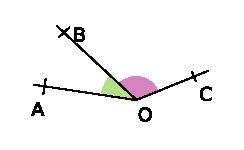
\includegraphics[width=.25\linewidth]{cours1}
\end{center}

\correction
Les angles $\widehat{AOB}$ et $\widehat{BOC}$ ont comme sommet commun le point $O$, comme côté commun la demi-droite $[OB)$ et sont placés de part et d'autre de $[OB)$ : ils sont donc adjacents.
\end{exemple*1}


\begin{exemple*1}
Sur la figure ci-dessous, que peux-tu dire des angles $\widehat{AOB}$ et $\widehat{DOE}$ ?

\begin{center}
    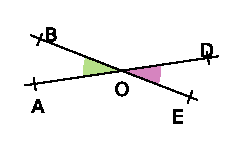
\includegraphics[width=.25\linewidth]{cours2}
\end{center}

\correction
Les angles $\widehat{AOB}$ et $\widehat{DOE}$ ont comme sommet commun le point $O$ et des côtés dans le prolongement l'un de l'autre ($A$, $O$, $D$ et $B$, $O$, $E$ sont alignés) : ils sont donc opposés par le sommet.
\end{exemple*1}

\vspace{1em}

Exercices « À toi de jouer »

Sur la figure ci-dessous, nomme trois paires d'angles adjacents.

\begin{center}
    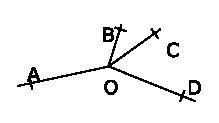
\includegraphics[width=.2\linewidth]{cours3}
\end{center}

Que dire des angles $\widehat{VST}$ et $\widehat{ESR}$ pour un parallélogramme $VERT$ de centre $S$ ?


\begin{aconnaitre}
Si deux angles sont opposés par le sommet \textbf{alors ils ont la même mesure.}
\end{aconnaitre}



\section{Angles complémentaires et supplémentaires}

\begin{aconnaitre}
\textbf{Deux angles complémentaires} sont deux angles dont la somme des mesures est égale à 90°.

\vspace{.5em}

\textbf{Deux angles supplémentaires} sont deux angles dont la somme des mesures est égale à 180°.
\end{aconnaitre}

\begin{exemple*1}
Sur la figure ci-dessous, que peux-tu dire des angles $\widehat{AOB}$ et $\widehat{BOC}$ ?

\begin{center}
    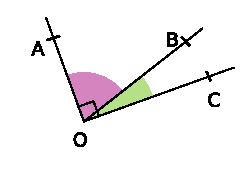
\includegraphics[width=.25\linewidth]{cours4}
\end{center}

\correction
Les angles $\widehat{AOB}$ et $\widehat{BOC}$ forment un angle droit : la somme des mesures de ces angles vaut 90°. Ce sont donc des angles complémentaires.
\end{exemple*1}

\begin{remarque}
Deux angles complémentaires et adjacents forment un angle droit. On peut donc en déduire que des droites sont perpendiculaires.
\end{remarque}


\begin{exemple*1}
Sur la figure ci-dessous, que peux-tu dire des angles $\widehat{AOB}$ et $\widehat{FED}$ ?

\begin{center}
    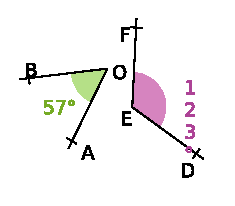
\includegraphics[width=.25\linewidth]{cours5}
\end{center}

\correction
$\widehat{AOB}+\widehat{FED}=57^\circ+123^\circ=180^\circ$ donc les angles $\widehat{AOB}$ et $\widehat{FED}$ sont supplémentaires.
\end{exemple*1}

\begin{remarque}
Deux angles supplémentaires et adjacents forment un angle plat. On peut donc en déduire que des points sont alignés.
\end{remarque}

\begin{remarque}
Deux angles complémentaires ou supplémentaires ne sont pas forcément adjacents.
\end{remarque}

\vspace{1em}

Exercices « À toi de jouer »

Les angles ci-dessous sont-ils complémentaires ?

\begin{center}
    
\includegraphics[width=.2\linewidth]{cours6}
\end{center}

Donne le complémentaire d'un angle de 27°.

Que peux-tu dire des angles aigus d'un triangle rectangle ? Justifie ta réponse.


Les angles ci-dessous sont-ils supplémentaires ?
\begin{center}
    
\includegraphics[width=.2\linewidth]{cours7}
\end{center}


Les points A, O et B sont-ils alignés ?
\begin{center}
    
\includegraphics[width=.2\linewidth]{cours8}
\end{center}







\section{Caractériser deux angles définis par deux droites et une sécante}


\begin{aconnaitre}
\begin{minipage}{.3\linewidth}
\centering

\includegraphics[width=.65\linewidth]{cours9}
\end{minipage}\hfill%
\begin{minipage}{.67\linewidth}
Les angles verts sont \textbf{alternes-internes}.

Ils sont déterminés par les droites $(d)$, $(d')$ et la sécante $(d_1)$.

Les angles roses sont \textbf{correspondants.}

Ils sont déterminés par les droites $(d)$, $(d')$ et la sécante $(d_2)$.
\end{minipage}
\end{aconnaitre}

\begin{exemple*1}
À l'aide de la figure, nomme des angles alternes-internes et des correspondants.

\begin{center}
    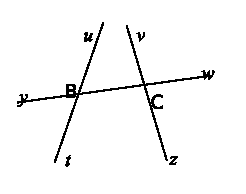
\includegraphics[width=.25\linewidth]{cours10}
\end{center}

\correction
Les droites $(ut)$, $(vz)$ et la sécante $(yw)$ forment :
\begin{itemize}
    \item deux paires d'angles alternes-internes qui sont : $\widehat{uBw}$ et $\widehat{yCz}$, $\widehat{vCy}$ et $\widehat{tBw}$.
    \item quatre paires d'angles correspondants qui sont : $\widehat{yBu}$ et $\widehat{vCy}$, $\widehat{yBt}$ et $\widehat{yCz}$, $\widehat{uBw}$ et $\widehat{vCw}$, $\widehat{tBw}$ et $\widehat{zCw}$.
\end{itemize}
\end{exemple*1}

\vspace{1em}

Exercices « À toi de jouer »

Sur la figure ci-dessous, les angles $\widehat{yOx'}$ et $\widehat{xEz'}$ sont-ils alternes-internes ? Justifie.

\begin{center}
    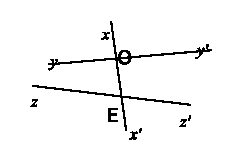
\includegraphics[width=.2\linewidth]{cours11}
\end{center}

Sur la figure  ci-dessous, nomme deux paires d'angles alternes-internes et quatre paires d'angles correspondants.

\begin{center}
    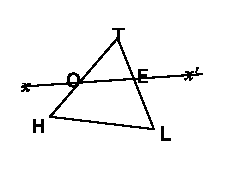
\includegraphics[width=.2\linewidth]{cours12}
\end{center}

\begin{aconnaitre}
Si deux angles alternes-internes sont déterminés par des droites parallèles \textbf{alors ils ont la même mesure.}

\vspace{.5em}

Si deux angles correspondants sont déterminés par des droites parallèles \textbf{alors ils ont la même mesure}.
\end{aconnaitre}

\begin{exemple*1}
Les droites $(vt)$ et $(uy)$ sont parallèles. Calcule la mesure des angles $\widehat{zEy}$ et $\widehat{vGw}$.

\begin{center}
    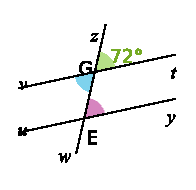
\includegraphics[width=.25\linewidth]{cours13}
\end{center}

\correction
Les angles correspondants $\widehat{zGt}$ et $\widehat{zEy}$ sont déterminés par les droites $(vt)$ et $(uy)$ qui sont parallèles. Ils sont donc de la même mesure. L'angle $\widehat{zEy}$ mesure donc 72°.

\vspace{.5em}

Les angles $\widehat{zGt}$ et $\widehat{vGw}$ sont opposés par le sommet. Ils sont donc de la même mesure. L'angle $\widehat{vGw}$ mesure donc 72°.
\end{exemple*1}

\vspace{1em}

Exercice « À toi de jouer »

Sur la figure ci-contre, les droites $(zz')$ et $(uu')$ sont parallèles. Calcule la mesure de l'angle $\widehat{x'Rz'}$ puis celle de l'angle $\widehat{uEx}$.

\begin{center}
    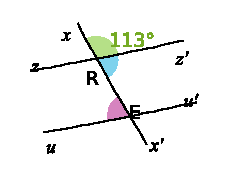
\includegraphics[width=.3\linewidth]{cours14}
\end{center}


\begin{aconnaitre}
Si deux angles alternes-internes sont de même mesure \textbf{alors les deux droites coupées par la sécante sont parallèles.}

\vspace{.5em}

Si deux angles correspondants sont de même mesure \textbf{alors les deux droites coupées par la sécante sont parallèles.}
\end{aconnaitre}


\begin{exemple*1}
Les droites $(yy')$ et $(zz')$ sont-elles parallèles ? Les droites $(xx')$ et $(uu')$ sont-elles parallèles ?

\begin{center}
    
\includegraphics[width=.3\linewidth]{cours15}
\end{center}

\correction
Les angles $\widehat{x'Ay'}$ et $\widehat{xBz}$ déterminés par les droites $(yy')$, $(zz')$ et la sécante $(xx')$ sont alternes-internes. Les angles $\widehat{x'Ay'}$ et $\widehat{xBz}$ ont la même mesure.

Donc les droites $(yy')$ et $(zz')$ sont parallèles.

\vspace{.5em}

Les angles $\widehat{x'Ay'}$ et $\widehat{u'Dy'}$ déterminés par les droites $(xx')$, $(uu')$ et la sécante $(yy')$ sont correspondants. Si les droites $(xx')$ et $(uu')$ étaient parallèles alors les angles $\widehat{x'Ay'}$ et $\widehat{u'Dy'}$ seraient de la même mesure, ce qui n'est pas le cas.

Donc les droites $(xx')$ et $(uu')$ ne sont pas parallèles.
\end{exemple*1}

\vspace{1em}

Exercice « À toi de jouer »

Dans chacun des cas ci-dessous, indique si les droites $(AB)$ et $(OT)$ sont parallèles. Justifie ta réponse.

\begin{center}
\begin{minipage}{.48\linewidth}
\centering
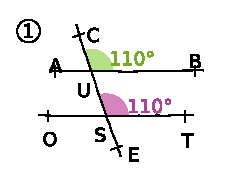
\includegraphics[width=.45\linewidth]{cours16}
\end{minipage}\hfill%
\begin{minipage}{.48\linewidth}
\centering
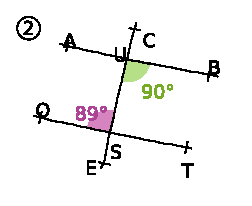
\includegraphics[width=.45\linewidth]{cours17}
\end{minipage}
\end{center}
